% !TEX TS-program = xelatex
% !TEX encoding = UTF-8 Unicode
% -*- coding: UTF-8; -*-
% vim: set fenc=utf-8

%%%%%%%%%%%%%%%%%%%%%%%%%%%%%%%%%%%%%%%%%%%%%%%%%%%%%%%%%%%%%%%%%
%% SIMPLE-THESIS-DISSERTATION
%% <https://github.com/zachscrivena/simple-thesis-dissertation>
%% This is free and unencumbered software released into the
%% public domain; see <http://unlicense.org> for details.
%%%%%%%%%%%%%%%%%%%%%%%%%%%%%%%%%%%%%%%%%%%%%%%%%%%%%%%%%%%%%%%%%

% See "README.md" for instructions on compiling this document.
\documentclass[letterpaper,nonstop,draftmode]{simplethesisdissertation}
\usepackage{tikz}
\usepackage{braket}
\usepackage{arev}
% Class options:
% a4paper, letterpaper, nonstop, draftmode.

%%%%%%%%%%%%%%%%%%%%%%%%%%%%%%%%%%%%%%%%%%%%%%%%%%%%%%%%%%%%%%%%%
%% PREAMBLE.
%%%%%%%%%%%%%%%%%%%%%%%%%%%%%%%%%%%%%%%%%%%%%%%%%%%%%%%%%%%%%%%%%

% Document properties.
\def\DocumentTitle{Insert Thesis Title Here}
\def\AuthorName{Insert Author Name Here}

% PDF settings and properties.
\hypersetup{
pdftitle={\DocumentTitle},
pdfauthor={\AuthorName},
pdfsubject={Ph.D. Thesis, University Institute of College, 2016},
pdfcreator={XeLaTeX},
pdfproducer={},
pdfkeywords={},
unicode=true,
bookmarks=true,
bookmarksopen=true,
pdfstartview=FitH,
pdfpagelayout=OneColumn,
pdfpagemode=UseOutlines,
hidelinks,
breaklinks,
bookmarksnumbered}

% Macros:
\DeclareMathOperator*{\argmax}{arg\,max}
\DeclareMathOperator*{\argmin}{arg\,min}
\renewcommand{\binom}[2]{\left(\genfrac{}{}{0pt}{}{#1}{#2}\right)}
\newcommand{\ceil}[1]{{\left\lceil{#1}\right\rceil}}
%\newcommand{\ffrac}[2]{{\nicefrac{#1}{#2}}}
%\newcommand{\fffrac}[2]{{\left.{#1}\middle/{#2}\right.}}
\newcommand{\floor}[1]{{\left\lfloor{#1}\right\rfloor}}
\DeclareMathOperator{\lcm}{lcm}
\newcommand{\ZZ}{{\mathbb{Z}}}

%%%%%%%%%%%%%%%%%%%%%%%%%%%%%%%%%%%%%%%%%%%%%%%%%%%%%%%%%%%%%%%%%
%% ACTUAL DOCUMENT.
%%%%%%%%%%%%%%%%%%%%%%%%%%%%%%%%%%%%%%%%%%%%%%%%%%%%%%%%%%%%%%%%%

\begin{document}

% Use Roman numerals (i, ii, iii, etc.) for page numbers in the front matter.
\pagenumbering{roman}

%%%%%%%%%%%%%%%%%%%%%%%%%%%%%%%%%%%%%%%%%%%%%%%%%%%%%%%%%%%%%%%%%
%% TITLE PAGE.
%%%%%%%%%%%%%%%%%%%%%%%%%%%%%%%%%%%%%%%%%%%%%%%%%%%%%%%%%%%%%%%%%

% No headers or footers on the title page.
\thispagestyle{empty}

\begingroup
\centering
\setstretch{1.0}
~
\\[1em]
\sffamily\bfseries\fontsize{26}{31.2}\selectfont
\DocumentTitle
\\[0.6in]
\sffamily\bfseries\Large
\AuthorName
\\[0.6in]
\normalfont\normalsize
An undergraduate thesis advised by Dr. David Craig \\~\\
submitted to the Department of Physics, Oregon State University \\~\\
in partial fulfillment of the requirements for the degree BSc in Physics \\[0.6in]
Submitted on May 8, 2020
\vfill

\includegraphics[height=1.0in]
{Figure-SchoolLogo}
\par
\endgroup

\clearpage

%%%%%%%%%%%%%%%%%%%%%%%%%%%%%%%%%%%%%%%%%%%%%%%%%%%%%%%%%%%%%%%%%
%% COPYRIGHT PAGE.
%%%%%%%%%%%%%%%%%%%%%%%%%%%%%%%%%%%%%%%%%%%%%%%%%%%%%%%%%%%%%%%%%

% \pagestyle{plain}
% \setcounter{page}{2}
%
% \begingroup
% \centering
% \setstretch{1.0}
% \null
% \vfill
% {\sffamily\textcopyright}~2016
% \\[0.5em]
% \AuthorName
% \\[0.5em]
% All Rights Reserved
% \par
% \endgroup
%
% \clearpage

% %%%%%%%%%%%%%%%%%%%%%%%%%%%%%%%%%%%%%%%%%%%%%%%%%%%%%%%%%%%%%%%%%
% %% DEDICATION PAGE.
% %%%%%%%%%%%%%%%%%%%%%%%%%%%%%%%%%%%%%%%%%%%%%%%%%%%%%%%%%%%%%%%%%
%
% \begingroup
% \centering
% \setstretch{1.0}
% ~
% \\[1in]
% \textit{Insert dedication here}
% \par
% \endgroup
%
% \clearpage

%%%%%%%%%%%%%%%%%%%%%%%%%%%%%%%%%%%%%%%%%%%%%%%%%%%%%%%%%%%%%%%%%
%% ACKNOWLEDGMENTS.
%%%%%%%%%%%%%%%%%%%%%%%%%%%%%%%%%%%%%%%%%%%%%%%%%%%%%%%%%%%%%%%%%

\chapter*{Acknowledgments}
\addcontentsline{toc}{chapter}{Acknowledgments}

I would like to thank Dr. David Craig, for guiding me through an engaging line of research, as well as Dr. David McIntyre, Dr. Elizabeth Gire, Dr. Corinne Manogue and Dr. Janet Tate for developing the quantum curriculum from which this thesis is rooted.

I would also like to thank all of those who gave me the time, space, and support I needed while writing this. This includes (but is certainly not limited to) my partner Brooke, my parents Joy and Kevin, my housemate Cheyanne, the staff of Interzone, and my friends Saskia, Rachel and Justin.

\clearpage

%%%%%%%%%%%%%%%%%%%%%%%%%%%%%%%%%%%%%%%%%%%%%%%%%%%%%%%%%%%%%%%%%
%% ABSTRACT.
%%%%%%%%%%%%%%%%%%%%%%%%%%%%%%%%%%%%%%%%%%%%%%%%%%%%%%%%%%%%%%%%%

\chapter*{Abstract}
\addcontentsline{toc}{chapter}{Abstract}

Standard quantum mechanics makes foundational assumptions to describe the measurement process. Upon interaction with a ``classical measurement apparatus'', a quantum system is subjected to postulated ``state collapse'' dynamics. We show that framing measurement around state collapse and ill-defined classical observers leads to interpretational issues, and artificially limits the scope of quantum theory. This motivates describing measurement as a unitary process instead. In the context of the Stern-Gerlach experiment, the measurement of an electron's spin angular momentum is explained as the entanglement of its spin and position degrees of freedom. Furthermore, the electron-environment interaction is also detailed as part of the measurement process. The environment plays the role of a record keeper, establishing the ``facts of the universe'' to make the measurement's occurrence objective. This enables the assignment of probabilities to outcomes of consecutive Stern-Gerlach experiments, which is done using the consistent histories approach to quantum mechanics. We exemplify how consistent histories can be used to give a unitary measurement model predictive power by reproducing the predictions of the standard approach. In doing so, we provide a ``spins-first'' introduction to the consistent histories approach that is targeted towards anybody looking to learn more about quantum foundations. Along the way, we coin a mathematically convenient operator that simplifies the calculation of probabilities. We conclude by discussing how consistent histories ignores the ``problem of outcomes'' in quantum measurement theory, and the connection between this problem and the many worlds interpretation of quantum mechanics.

% A novel approach to limiting extraneous predictions implements the principle of complementarity into the measurement process directly.

\clearpage

%%%%%%%%%%%%%%%%%%%%%%%%%%%%%%%%%%%%%%%%%%%%%%%%%%%%%%%%%%%%%%%%%
%% TABLE OF CONTENTS (TOC), LISTS OF FIGURES, TABLES, ETC.
%%%%%%%%%%%%%%%%%%%%%%%%%%%%%%%%%%%%%%%%%%%%%%%%%%%%%%%%%%%%%%%%%

\tableofcontents

\listoffigures

\clearpage

% Use Arabic numerals (1, 2, 3, etc.) for subsequent page numbers.
\pagenumbering{arabic}


\usetikzlibrary{shapes.geometric}
\usetikzlibrary{positioning}

\newcommand{\apparatus}[4]{\node[square node] (#1) at (#2,#3){#4};
                           \node[port] (#1+) at (#2 + 0.375, #3 + 0.5){+};
                           \node[port] (#1-) at (#2 + 0.375, #3 - 0.5){-};}

\part{Background}
\chapter{Stern-Gerlach Experiments}
\section{Stern-Gerlach Backgorund}
TODO
\section{Stern-Gerlach Measurement}

We begin by comparing standard and consistent descriptions of measuring a quantum states' spin along one axis using a Stern-Gerlach apparatus. In standard quantum mechanics, the act of measurement plays a special role in assigning probabilities to the outcome and the evolution of the state through the probability and projection postulates.

The probability postulate assigns probabilities to each measurement by taking the inner product of the state $\ket{n}$ corresponding to a measruement result $n$ and $\ket{\psi}$:
\begin{align}
    \mathcal{P}_n = |\braket{n|\psi}|^2
\end{align}

The projection postulate describes an instantaneous evolution of the input state to an output state that corresponds to an allowed measruement value. If input $\ket{\psi}$ is measured to have spin $n$ (up or down), then the new state is
\begin{align}
    \ket{\psi}^\prime = \frac{P_n\ket{\psi}}{\sqrt{\bra{\psi}P_n\ket{\psi}
    }}
\end{align}
where $P_n = \ket{n}\bra{n}$ is the projection operator for state $\ket{n}$. This operation projects $\ket{\psi}$ onto $\ket{n}$, then divides by the magnitude of that projection. The end result is that $\ket{\psi}$ becomes the normalized state $\ket{n}$ corresponding to measuring spin $n$, which is shown by the states exiting the each apparatus.

\begin{figure}
\centering\CaptionFontSize
\begin{tikzpicture}[shorten >=1pt,auto, thick,
     square node/.style={rectangle, minimum height=2cm, minimum width=1.50cm, text width = 1.25cm, draw, font=\sffamily\Large\bfseries},
     port/.style={rectangle, draw,  minimum height=1cm, minimum width=0.75cm, font=\sffamily\Large\bfseries},
     wf/.style={rectangle, minimum height=1cm}]
    \apparatus{1}{3}{0}{$Z$};
    \apparatus{2}{6}{1.5}{$X$};

    \node[wf] (w0) at (0,0) {$\ket{\psi}$};
    \node[wf] (w1) at (8, 2.0) {$\ket{+}_x$};
    \node[wf] (w2) at (8, 1.0) {$\ket{-}_x$};

    \draw[line width=0.5mm] (w0) -- (1);

    \draw[line width=0.5mm] (1+) -- (2) node [near end] {$\ket{+}$};

    \draw[line width=0.5mm] (2+) -- (w1);
    \draw[line width=0.5mm] (2-) -- (w2);
\end{tikzpicture}
\caption[Insert an abbreviated caption here to show in the List of Figures]
{Demonstrating renormalizing upon measurment in standard quantum mechanics}
\label{Figure:Intro:FigureExampleA}
\end{figure}

TODO: show probability computations
TODO: explain how measurement is not itself modeled as a physical process, and we are directed to use these postulates upon poorly defined "measurement"

In consistent quantum theory, measurement is modeled as a physical process. Each Stern-Gerlach apparatus has its own detector Hilbert space, containing orthonormal states representing each measurement result. Let the state space of the $z$ apparatus be represented by ${\mathcal{H}_D}_z =  \{\ket{D_z}_+, \ket{D_z}_-\}$ where $_+\braket{D_z|D_z}_+=1$ and $_+\braket{D_z|D_z}_-=0$. ${\mathcal{H}_D}_x$ is similarly defined. Each detector state is orthogonal to states in seperate detector spaces.

The act of measurement is described by correlating the detector states with the corresponding quantum states. The system then evolves by
\begin{align}
    \nonumber V: \\
    & \nonumber \mathcal{H}_s \mapsto \mathcal{H}_s \otimes \mathcal{H}_D \\
    & \ket{\psi} = \sum_{n} P_n\ket{\psi} \mapsto \sum_{n} P_n\ket{\psi} \otimes \ket{D}_n
\end{align}

Measurment is now described by an abstract physical process. In this model, it is now feasible for "state collapse" to occur independent of physicists conducting clever experiments.

To compute probabilities of each outcome, we sum the magnitudes of each branch wavefunction that includes the corresponding detector state. This is accomplished by finding the trace of the projection operator of that detector state acting on the projection operator or the overall evolved state.
\begin{align}
    \mathcal{P}_n = Tr(P^D_n \cdot V\ket{\psi}\bra{\psi}V^\dagger)
\end{align}

In this simple Stern-Gerlach example, there is only one branch wavefunction correlated with each detector state. So, computing probabilities is done by finding the magnitude of each branch wavefunction.

TODO: compute probabilities, show it is equal to std QM

\begin{figure}
\centering\CaptionFontSize
\begin{tikzpicture}[shorten >=1pt,auto, thick,
     square node/.style={rectangle, minimum height=2cm, minimum width=1.50cm, text width = 1.25cm, draw, font=\sffamily\Large\bfseries},
     port/.style={rectangle, draw,  minimum height=1cm, minimum width=0.75cm, font=\sffamily\Large\bfseries},
     wf/.style={rectangle, minimum height=1cm, text width = 0.7cm}]
    \apparatus{1}{3}{0}{$Z$};
    \apparatus{2}{6}{1.5}{$X$};

    \node[wf] (w0) at (0,0) {$\ket{\psi}$};
    \node[wf] (w1) at (8, 2.0) {$P^x_+ \ket{+} \otimes \ket{D_z}_+  \otimes \ket{D_x}_+$};
    \node[wf] (w2) at (8, 1.0) {$P^x_- \ket{+} \otimes \ket{D_z}_+ \otimes \ket{D_x}_-$};

    \draw[line width=0.5mm] (w0) -- (1);

    \draw[line width=0.5mm] (1+) -- (2) node [near end] {$\ket{+} \otimes \ket{D_z}_+$};

    \draw[line width=0.5mm] (2+) -- (w1);
    \draw[line width=0.5mm] (2-) -- (w2);
\end{tikzpicture}
\caption[Insert an abbreviated caption here to show in the List of Figures]
{Demonstrating description of measurment as an abstract physical process in consistent quantum mechanics}
\label{Figure:Intro:FigureExampleB}
\end{figure}

\section{Complementarity}

We now compare standard and consistent quantum mechanics' treatment of the principle of complementarity. Arguably the most fundamental feature of quantum mechanics, the principle of complementarity states that a quantum system has pairs of physical observables which cannot be measured simultaneously. Components of spin on orthogonal axes are complemntary properties, so we examine measurements of succesive Stern-Gerlach experiments.

First, we compute the probabilities of each outcome using standard quantum mechanics. The first apparatus serves as a state preparation device with output $\ket{+}$. By the direction of the projection postulate, the state is renormalized upon each measruement. After measuring a property complementary to what is known (such as spin along $x$, knowing spin along $z$), any information known about the input state is lost; the input state instantaneously changes to the state corresponding to the observed quantity. Consequently, there is an equal probability of observing the final state as $\ket{+}$ or $\ket{-}$ at either final apparatus, even though the state was initially prepared as $\ket{+}$, since
\begin{align*}
    \mathcal{P}_n &= |\braket{+|+}_x|^2 \\
                  &= |\braket{-|+}_x|^2 \\
                  &= |\braket{+|-}_x|^2 \\
                  &= |\braket{-|-}_x|^2 \\
                  &= \frac{1}{4}
\end{align*}
This contradiction with classical intuition is a direct result of the projection postulate. TODO: describe measurement problem.

TODO: Demonstrate complementarity and single framework rule

\begin{figure}
\centering\CaptionFontSize
\begin{tikzpicture}[shorten >=1pt,auto, thick,
     square node/.style={rectangle, minimum height=2cm, minimum width=1.50cm, text width = 1.25cm, draw, font=\sffamily\Large\bfseries},
     port/.style={rectangle, draw,  minimum height=1cm, minimum width=0.75cm, font=\sffamily\Large\bfseries},
     wf/.style={rectangle, minimum height=1cm}]
    \apparatus{1}{3}{0}{$Z$};
    \apparatus{2}{6}{1.25}{$X$};
    \apparatus{3}{9}{2.50}{$Z$};
    \apparatus{4}{9}{0}{$Z$};

    \node[wf] (w0) at (0,0) {$\ket{\psi}$};
    \node[wf] (w1) at (11, 3.0) {$\ket{+}$};
    \node[wf] (w2) at (11, 2.0) {$\ket{-}$};
    \node[wf] (w3) at (11, 0.5) {$\ket{+}$};
    \node[wf] (w4) at (11, -0.5) {$\ket{-}$};

    \draw[line width=0.5mm] (w0) -- (1);

    \draw[line width=0.5mm] (1+) -- (2) node [near end] {$\ket{+}$};

    \draw[line width=0.5mm] (2-) -- (4) node [midway, below] {$\ket{-}_x$};
    \draw[line width=0.5mm] (2+) -- (3) node [midway, above] {$\ket{+}_x$};

    \draw[line width=0.5mm] (3-) -- (w2);
    \draw[line width=0.5mm] (3+) -- (w1);
    \draw[line width=0.5mm] (4-) -- (w4);
    \draw[line width=0.5mm] (4+) -- (w3);
\end{tikzpicture}
\caption[Insert an abbreviated caption here to show in the List of Figures]
{Demonstrating complementary measurments in standard quantum mechanics}
\label{Figure:Intro:FigureExampleC}
\end{figure}

\begin{figure}
\centering\CaptionFontSize
\begin{tikzpicture}[shorten >=1pt,auto, thick,
     square node/.style={rectangle, minimum height=2cm, minimum width=1.50cm, text width = 1.25cm, draw, font=\sffamily\Large\bfseries},
     port/.style={rectangle, draw,  minimum height=1cm, minimum width=0.75cm, font=\sffamily\Large\bfseries},
     wf/.style={rectangle, minimum height=1cm}]
    \apparatus{1}{3}{0}{$Z$};
    \apparatus{2}{6}{1.25}{$X$};
    \apparatus{3}{9}{2.50}{$Z$};
    \apparatus{4}{9}{0}{$Z$};

    \node[wf] (w0) at (0,0) {$\ket{\psi}$};
    \node[wf] (w1) at (11, 3.0) {$\ket{+}$};
    \node[wf] (w2) at (11, 2.0) {$\ket{-}$};
    \node[wf] (w3) at (11, 0.5) {$\ket{+}$};
    \node[wf] (w4) at (11, -0.5) {$\ket{-}$};

    \draw[line width=0.5mm] (w0) -- (1);

    \draw[line width=0.5mm] (1+) -- (2) node [near end] {$\ket{+}$};

    \draw[line width=0.5mm] (2-) -- (4) node [midway, below] {$\ket{-}_x$};
    \draw[line width=0.5mm] (2+) -- (3) node [midway, above] {$\ket{+}_x$};

    \draw[line width=0.5mm] (3-) -- (w2);
    \draw[line width=0.5mm] (3+) -- (w1);
    \draw[line width=0.5mm] (4-) -- (w4);
    \draw[line width=0.5mm] (4+) -- (w3);
\end{tikzpicture}
\caption[Insert an abbreviated caption here to show in the List of Figures]
{Demonstrating complementary measurments in consistent quantum mechanics}
\label{Figure:Intro:FigureExampleD}
\end{figure}

\begin{figure}
\centering\CaptionFontSize
\begin{tikzpicture}[shorten >=1pt,auto, thick,
     square node/.style={rectangle, minimum height=2cm, minimum width=1.50cm, text width = 1cm, draw, font=\sffamily\Large\bfseries},
     port/.style={rectangle, draw,  minimum height=1cm, minimum width=0.75cm, font=\sffamily\Large\bfseries},
     wf/.style={rectangle, minimum height=1cm}]
    \apparatus{1}{3}{0}{Z};
    \apparatus{2}{6}{1}{X};
    \apparatus{3}{9}{1}{Z};

    \node[wf] (w0) at (0,0) {$\ket{\psi}$};
    \node[wf] (w1) at (12,2.5) {$\ket{\psi_1}$};
    \node[wf] (w2) at (12,1.5) {$\ket{\psi_2}$};
    \node[wf] (w3) at (12,0.5) {$\ket{\psi_3}$};
    \node[wf] (w4) at (12,-0.5) {$\ket{\psi_4}$};

    \draw[line width=0.5mm] (w0) -- (1);

    \draw[transform canvas={yshift=-0.6em}, line width=0.5mm, loosely dotted] (1+) -- (2);
    \draw[transform canvas={yshift=-0.2em}, line width=0.5mm, dotted] (1+) -- (2);
    \draw[transform canvas={yshift=0.2em}, line width=0.5mm, dashed] (1+) -- (2);
    \draw[transform canvas={yshift=0.6em}, line width=0.5mm] (1+) -- (2);

    \draw[transform canvas={yshift=-0.4em}, line width=0.5mm, loosely dotted] (2-) -- (3);
    \draw[transform canvas={yshift=0em}, line width=0.5mm, dotted] (2-) -- (3);
    \draw[transform canvas={yshift=0em}, line width=0.5mm, dashed] (2+) -- (3);
    \draw[transform canvas={yshift=0.4em}, line width=0.5mm] (2+) -- (3);

    \draw[line width=0.5mm, loosely dotted] (3-) -- (w4);
    \draw[line width=0.5mm, dashed] (3-) -- (w3);
    \draw[line width=0.5mm, dotted] (3+) -- (w2);
    \draw[line width=0.5mm] (3+) -- (w1);
\end{tikzpicture}
\caption[Insert an abbreviated caption here to show in the List of Figures]
{TODO: create section to discuss this example, and how it creates an inconsistent set of histories. Describe how the set can be made to be consistent}
\label{Figure:Intro:FigureExampleE}
\end{figure}



\chapter{Insert Chapter Title Here}
\label{Section:ChapAbbr}

\BlankFootnote{Insert chapter footnote here.
The chapter footnote could include citations to related publications by the author (``The material in this chapter was presented in part in ....'').}

%%%%%%%%%%%%%%%%%%%%%%%%%%%%%%%%%%%%%%%%%%%%%%%%%%%%%%%%%%%%%%%%%
%%%%%%%%%%%%%%%%%%%%%%%%%%%%%%%%%%%%%%%%%%%%%%%%%%%%%%%%%%%%%%%%%
%%%%%%%%%%%%%%%%%%%%%%%%%%%%%%%%%%%%%%%%%%%%%%%%%%%%%%%%%%%%%%%%%

\section{Introduction}
\label{Section:ChapAbbr:Introduction}

Insert chapter introduction here.
\lipsum[1-2]

\mbox{\textit{Related Work:}}
Our work is related to \cite{Examples:Conference01, Examples:Journal01, Examples:Conference02, Examples:Journal02, Examples:Conference03}.
\lipsum[3-4]

\mbox{\textit{Our Contribution:}}
\lipsum[5-6]

Proofs of theorems are deferred to \Section~\sref{Section:ChapAbbr:ProofsOfTheorems}.

%%%%%%%%%%%%%%%%%%%%%%%%%%%%%%%%%%%%%%%%%%%%%%%%%%%%%%%%%%%%%%%%%
%%%%%%%%%%%%%%%%%%%%%%%%%%%%%%%%%%%%%%%%%%%%%%%%%%%%%%%%%%%%%%%%%
%%%%%%%%%%%%%%%%%%%%%%%%%%%%%%%%%%%%%%%%%%%%%%%%%%%%%%%%%%%%%%%%%

\section{Some Examples}
\label{Section:ChapAbbr:SomeExamples}

\lipsum[7]

%%%%%%%%%%%%%%%%%%%%%%%%%%%%%%%%%%%%%%%%%%%%%%%%%%%%%%%%%%%%%%%%%
%%%%%%%%%%%%%%%%%%%%%%%%%%%%%%%%%%%%%%%%%%%%%%%%%%%%%%%%%%%%%%%%%
%%%%%%%%%%%%%%%%%%%%%%%%%%%%%%%%%%%%%%%%%%%%%%%%%%%%%%%%%%%%%%%%%

\subsection{Examples of Figures and Tables}
\label{Section:ChapAbbr:SomeExamples:FiguresTables}

%%%%%%%%%%%%%%%%%%%%%%%%%%%%%%%%%%%%%%%%%%%%%%%%%%%%%%%%%%%%%%%%%
% FIGURE: CHAPABBR: FIGURE EXAMPLE A
\begin{figure}
\centering\CaptionFontSize
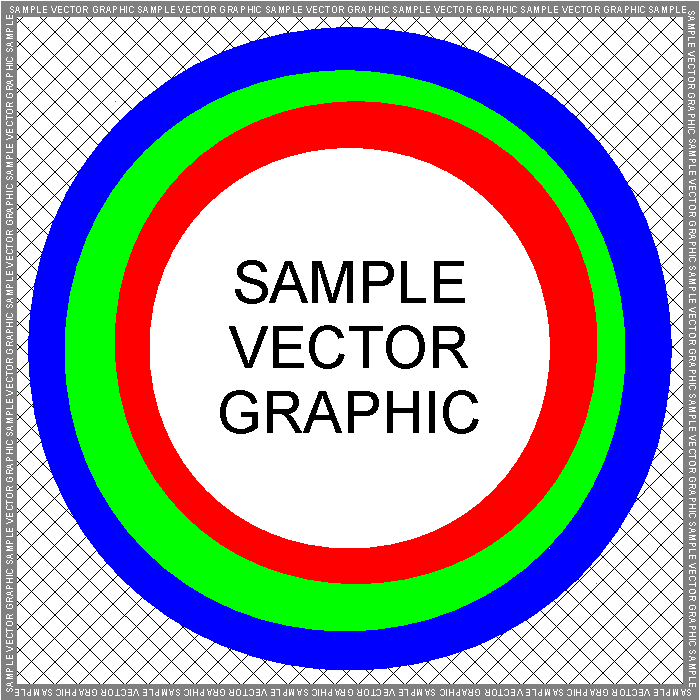
\includegraphics[height=15em]
{Figure-ChapAbbr-FigureExampleA}
\caption[Insert an abbreviated caption here to show in the List of Figures]
{Insert the full caption here for this floating figure.}
\label{Figure:ChapAbbr:FigureExampleA}
\end{figure}
%%%%%%%%%%%%%%%%%%%%%%%%%%%%%%%%%%%%%%%%%%%%%%%%%%%%%%%%%%%%%%%%%

This is a reference to \Figure~\fref{Figure:ChapAbbr:FigureExampleA}.
\lipsum[8]

%%%%%%%%%%%%%%%%%%%%%%%%%%%%%%%%%%%%%%%%%%%%%%%%%%%%%%%%%%%%%%%%%
% FIGURE: CHAPABBR: FIGURE EXAMPLE B
\begin{sidewaysfigure*}
\centering\CaptionFontSize
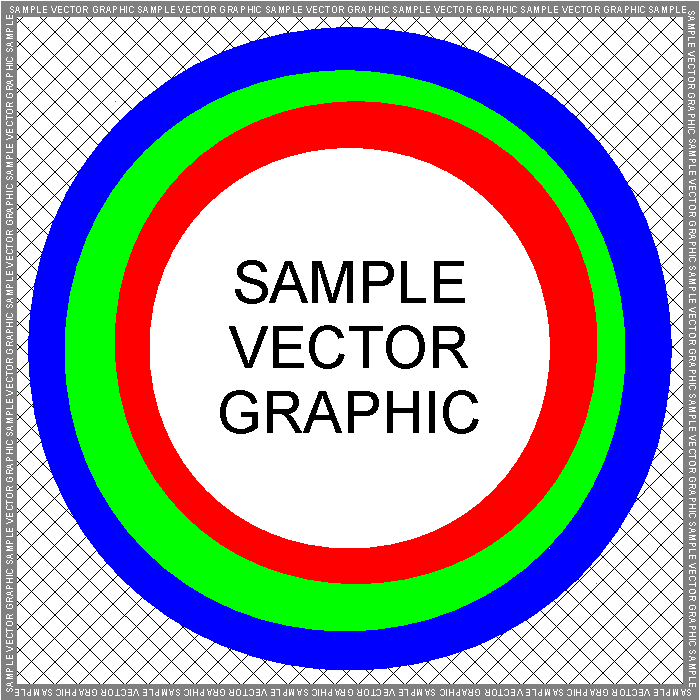
\includegraphics[height=30em]
{Figure-ChapAbbr-FigureExampleB}
\caption[Insert an abbreviated caption here to show in the List of Figures]
{Insert the full caption here for this floating figure.
The caption should provide sufficient context to interpret the figure.
Lorem ipsum dolor sit amet, consectetuer adipiscing elit.
Ut purus elit, vestibulum ut, placerat ac, adipiscing vitae, felis.
Curabitur dictum gravida mauris.}
\label{Figure:ChapAbbr:FigureExampleB}
\end{sidewaysfigure*}
%%%%%%%%%%%%%%%%%%%%%%%%%%%%%%%%%%%%%%%%%%%%%%%%%%%%%%%%%%%%%%%%%

Here we say something about \Figures~\fref{Figure:ChapAbbr:FigureExampleA} and~\fref{Figure:ChapAbbr:FigureExampleB}.
Note how the effect in \Figure~\fref{Figure:ChapAbbr:FigureExampleB} is stronger that in \Figure~\fref{Figure:ChapAbbr:FigureExampleA}.
\lipsum[9]

%%%%%%%%%%%%%%%%%%%%%%%%%%%%%%%%%%%%%%%%%%%%%%%%%%%%%%%%%%%%%%%%%
% TABLE: CHAPABBR: EXAMPLE A
\begin{table}
\caption[Insert an abbreviated caption here to show in the List of Tables]
{Insert the full caption here for this floating table.}
\label{Table:ChapAbbr:TableExampleA}
\centering\CaptionFontSize
\begin{tabular}{c@{\hspace{1em}}l}
\toprule
Symbol & Definition
\\
\midrule
$\alpha$ & insert definition of $\alpha$ here, $\alpha\geq 1$
\\
$\beta$ & insert definition of $\beta$ here, $\beta\geq 2$
\\
$\gamma$ & insert definition of $\gamma$ here, $\gamma\geq 3$
\\
$\delta$ & insert definition of $\delta$ here, $\delta\geq 4$
\\
\bottomrule
\end{tabular}
\end{table}
%%%%%%%%%%%%%%%%%%%%%%%%%%%%%%%%%%%%%%%%%%%%%%%%%%%%%%%%%%%%%%%%%

We summarize our notation in \Table~\tref{Table:ChapAbbr:TableExampleA}.
\lipsum[10]

%%%%%%%%%%%%%%%%%%%%%%%%%%%%%%%%%%%%%%%%%%%%%%%%%%%%%%%%%%%%%%%%%
% TABLE: CHAPABBR: EXAMPLE B
\begin{table}
\caption[Insert an abbreviated caption here to show in the List of Tables]
{Insert the full caption here for this floating table.
The caption should provide sufficient context to interpret the table.
Lorem ipsum dolor sit amet, consectetuer adipiscing elit.
Ut purus elit, vestibulum ut, placerat ac, adipiscing vitae, felis.
Curabitur dictum gravida mauris.}
\label{Table:ChapAbbr:TableExampleB}
\centering\CaptionFontSize
\begin{tabular}{c@{\hspace{1em}}l@{\hspace{1em}}c}
\toprule
Variable & Initial Value & Value at $t=100$
\\
\midrule
$c$ & $0.012$ & $3.456$
\\
$\delta$ & $0.312$ & $1.416$
\\
$\gamma$ & $0.042$ & $3.252$
\\
$h$ & $0.012$ & $3.353$
\\
$c$ & $0.012$ & $4.446$
\\
$\delta$ & $0.015$ & $3.556$
\\
$\gamma$ & $0.612$ & $6.656$
\\
$h$ & $0.072$ & $7.456$
\\
$c$ & $0.018$ & $8.756$
\\
$\delta$ & $0.912$ & $9.456$
\\
$\gamma$ & $0.092$ & $5.956$
\\
$h$ & $0.012$ & $2.326$
\\
\bottomrule
\end{tabular}
\end{table}
%%%%%%%%%%%%%%%%%%%%%%%%%%%%%%%%%%%%%%%%%%%%%%%%%%%%%%%%%%%%%%%%%

\Table~\tref{Table:ChapAbbr:TableExampleB} summarizes our simulation results.
\lipsum[11]

%%%%%%%%%%%%%%%%%%%%%%%%%%%%%%%%%%%%%%%%%%%%%%%%%%%%%%%%%%%%%%%%%

\subsection{Examples of Enumerated and Itemized Lists}
\label{Section:ChapAbbr:SomeExamples:Lists}

Here are some citations \cite{Examples:Conference03, Examples:Journal03, Examples:Conference04, Examples:Journal04, Examples:Conference05, Examples:Journal05}.
The following is an enumerated list, or numbered list, with multiple levels:

%%%%%%%%%%%%%%%%%%%%%%%%%%%%%%%%%%%%%%%%%%%%%%%%%%%%%%%%%%%%%%%%%
\begin{enumerate}
\item
\label{Item:ChapAbbr:ItemExampleA}
First level item
\item
First level item
\begin{enumerate}
\item
Second level item
\item
Second level item
\begin{enumerate}
\item
Third level item
\begin{enumerate}
\item
Fourth level item
\item
Fourth level item
\end{enumerate}
\item
Third level item
\end{enumerate}
\item
Second level item
\end{enumerate}
\item
\label{Item:ChapAbbr:ItemExampleB}
First level item
\end{enumerate}
%%%%%%%%%%%%%%%%%%%%%%%%%%%%%%%%%%%%%%%%%%%%%%%%%%%%%%%%%%%%%%%%%

We draw your attention to items \ref{Item:ChapAbbr:ItemExampleA} and \ref{Item:ChapAbbr:ItemExampleB} in particular because they are very important in our study.
The following is an itemized list, or unnumbered list, with multiple levels:

%%%%%%%%%%%%%%%%%%%%%%%%%%%%%%%%%%%%%%%%%%%%%%%%%%%%%%%%%%%%%%%%%
\begin{itemize}
\item
First level item
\item
First level item
\begin{itemize}
\item
Second level item
\item
Second level item
\begin{itemize}
\item
Third level item
\begin{itemize}
\item
Fourth level item
\item
Fourth level item
\end{itemize}
\item
Third level item
\end{itemize}
\item
Second level item
\end{itemize}
\item
First level item
\end{itemize}
%%%%%%%%%%%%%%%%%%%%%%%%%%%%%%%%%%%%%%%%%%%%%%%%%%%%%%%%%%%%%%%%%

%%%%%%%%%%%%%%%%%%%%%%%%%%%%%%%%%%%%%%%%%%%%%%%%%%%%%%%%%%%%%%%%%
%%%%%%%%%%%%%%%%%%%%%%%%%%%%%%%%%%%%%%%%%%%%%%%%%%%%%%%%%%%%%%%%%
%%%%%%%%%%%%%%%%%%%%%%%%%%%%%%%%%%%%%%%%%%%%%%%%%%%%%%%%%%%%%%%%%

\section{Some More Examples}
\label{Section:ChapAbbr:SomeMoreExamples}

According to~\cite{IEEEexample:book_typical}, this behavior can be explained this way.
\lipsum[12]

%%%%%%%%%%%%%%%%%%%%%%%%%%%%%%%%%%%%%%%%%%%%%%%%%%%%%%%%%%%%%%%%%
%%%%%%%%%%%%%%%%%%%%%%%%%%%%%%%%%%%%%%%%%%%%%%%%%%%%%%%%%%%%%%%%%
%%%%%%%%%%%%%%%%%%%%%%%%%%%%%%%%%%%%%%%%%%%%%%%%%%%%%%%%%%%%%%%%%

\subsection{Examples of Mathematical Expressions, Definitions, and Theorems}
\label{Section:ChapAbbr:SomeMoreExamples:Math}

We have the following unnumbered mathematical equation:
\[
E=mc^2.
\]
On the other hand, the following is a numbered mathematical inequality:
%%%%%%%%%%%%%%%%%%%%%%%%%%%%%%%%%%%%%%%%%%%%%%%%%%%%%%%%%%%%%%%%%
\begin{align}
x \leq
\frac{\displaystyle\sum_{i=1}^{n} y^2 \cdot \one{y > 1}}
{\displaystyle\int_{-\infty}^{\infty} x^3 \;\text{d}z \cdot
\binom{\alpha}{\beta} \frac{\floor{\frac{a}{b}}}{\ceil{\frac{c}{d}}}}.
\label{Eq:ChapAbbr:EqExampleA}
\end{align}
%%%%%%%%%%%%%%%%%%%%%%%%%%%%%%%%%%%%%%%%%%%%%%%%%%%%%%%%%%%%%%%%%
Inequality~\eqref{Eq:ChapAbbr:EqExampleA} will be applied multiple times to prove our theorems, in a manner similar to \cite{IEEEexample:article_typical, IEEEexample:conf_typical}.
We now introduce the following definition:

\begin{Thm:Definition}[Name of Term Being Defined]
This is the definition of the term, along with relevant conditions, trivial cases, exceptions, etc.
\end{Thm:Definition}

We can rewrite the result of \cite[Theorem~2.5]{IEEEexample:conf_typical} in the following convenient form for our problem:

%%%%%%%%%%%%%%%%%%%%%%%%%%%%%%%%%%%%%%%%%%%%%%%%%%%%%%%%%%%%%%%%%
\begin{Thm:Proposition}
For all \mbox{$a,b,c\in\ZZ^+$}, we have
\label{Thm:Proposition:ChapAbbr:PropositionExample}
\[
a^2+b^3\leq c^4.
\]
\end{Thm:Proposition}
%%%%%%%%%%%%%%%%%%%%%%%%%%%%%%%%%%%%%%%%%%%%%%%%%%%%%%%%%%%%%%%%%

Based on our numerical observations, we make the following conjecture about the upper bound:

%%%%%%%%%%%%%%%%%%%%%%%%%%%%%%%%%%%%%%%%%%%%%%%%%%%%%%%%%%%%%%%%%
\begin{Thm:Conjecture}
If \mbox{$x\geq 3$} and \mbox{$0<y<x^2$}, then for all \mbox{$n\in\ZZ^+$},
\[
\sum_{i=1}^{n} x_i
= x_1 + x_2 + \cdots + x_n
\leq T_{\textup{all}}.
\]
\end{Thm:Conjecture}
%%%%%%%%%%%%%%%%%%%%%%%%%%%%%%%%%%%%%%%%%%%%%%%%%%%%%%%%%%%%%%%%%

Here is a lemma that will be quite useful in deriving our results:

%%%%%%%%%%%%%%%%%%%%%%%%%%%%%%%%%%%%%%%%%%%%%%%%%%%%%%%%%%%%%%%%%
\begin{Thm:Lemma}
[Name of Lemma if any]
\label{Thm:Lemma:ChapAbbr:LemmaExampleA}
If \mbox{$x,y,z\in\ZZ^+_0$}, then \mbox{$f(x+y+z) = 1$}.
\end{Thm:Lemma}
%%%%%%%%%%%%%%%%%%%%%%%%%%%%%%%%%%%%%%%%%%%%%%%%%%%%%%%%%%%%%%%%%

Applying \Lemma~\mref{Thm:Lemma:ChapAbbr:LemmaExampleA} to \cite[Theorem~4.2]{IEEEexample:book_typical} produces the following theorem:

%%%%%%%%%%%%%%%%%%%%%%%%%%%%%%%%%%%%%%%%%%%%%%%%%%%%%%%%%%%%%%%%%
\begin{Thm:Theorem}
[Name of Theorem if any]
\label{Thm:Theorem:ChapAbbr:TheoremExample}
If \mbox{$x+y\geq z$}, then
\begin{align*}
\sum_{i=x}^{y} f(i) \leq z.
\end{align*}
\end{Thm:Theorem}
%%%%%%%%%%%%%%%%%%%%%%%%%%%%%%%%%%%%%%%%%%%%%%%%%%%%%%%%%%%%%%%%%

As a special case of \Theorem~\mref{Thm:Theorem:ChapAbbr:TheoremExample}, we have the following corollary:

%%%%%%%%%%%%%%%%%%%%%%%%%%%%%%%%%%%%%%%%%%%%%%%%%%%%%%%%%%%%%%%%%
\begin{Thm:Corollary}
If \mbox{$x=4$} and \mbox{$y=z$}, then \mbox{$\sum_{i=x}^{y} f(i) = 5$}.
\end{Thm:Corollary}
%%%%%%%%%%%%%%%%%%%%%%%%%%%%%%%%%%%%%%%%%%%%%%%%%%%%%%%%%%%%%%%%%

\lipsum[13]

%%%%%%%%%%%%%%%%%%%%%%%%%%%%%%%%%%%%%%%%%%%%%%%%%%%%%%%%%%%%%%%%%
%%%%%%%%%%%%%%%%%%%%%%%%%%%%%%%%%%%%%%%%%%%%%%%%%%%%%%%%%%%%%%%%%
%%%%%%%%%%%%%%%%%%%%%%%%%%%%%%%%%%%%%%%%%%%%%%%%%%%%%%%%%%%%%%%%%

\section{Conclusion and Future Work}
\label{Section:ChapAbbr:Conclusion}

\lipsum[14-15]

%%%%%%%%%%%%%%%%%%%%%%%%%%%%%%%%%%%%%%%%%%%%%%%%%%%%%%%%%%%%%%%%%
%%%%%%%%%%%%%%%%%%%%%%%%%%%%%%%%%%%%%%%%%%%%%%%%%%%%%%%%%%%%%%%%%
%%%%%%%%%%%%%%%%%%%%%%%%%%%%%%%%%%%%%%%%%%%%%%%%%%%%%%%%%%%%%%%%%

\section{Proofs of Theorems}
\label{Section:ChapAbbr:ProofsOfTheorems}

\noindent
{\color{red}%
Remember to manually disable (and re-enable) updates to the table of contents (TOC), using
\[
\verb|\DisableTOCUpdates|
\text{ and }
\verb|\EnableTOCUpdates|,
\]
if you want to omit subsections, tables, figures, etc., from the table of contents.}

%%%%%%%%%%%%%%%%%%%%%%%%%%%%%%%%%%%%%%%%%%%%%%%%%%%%%%%%%%%%%%%%%

\DisableTOCUpdates

%%%%%%%%%%%%%%%%%%%%%%%%%%%%%%%%%%%%%%%%%%%%%%%%%%%%%%%%%%%%%%%%%

\subsection{Proof of Lemma~\ref{Thm:Lemma:ChapAbbr:LemmaExampleA}}

\lipsum[16-17]
\qedmarker

%%%%%%%%%%%%%%%%%%%%%%%%%%%%%%%%%%%%%%%%%%%%%%%%%%%%%%%%%%%%%%%%%

\subsection{Proof of Theorem~\ref{Thm:Theorem:ChapAbbr:TheoremExample}}

\lipsum[18]

The following lemma will be quite useful in deriving the theorem:

%%%%%%%%%%%%%%%%%%%%%%%%%%%%%%%%%%%%%%%%%%%%%%%%%%%%%%%%%%%%%%%%%
\begin{Thm:Lemma}
\label{Thm:Lemma:ChapAbbr:LemmaExampleB}
If \mbox{$a,b,c\in\ZZ$}, then \mbox{$g(a\cdot b\cdot c) \leq -1$}.
\end{Thm:Lemma}
%%%%%%%%%%%%%%%%%%%%%%%%%%%%%%%%%%%%%%%%%%%%%%%%%%%%%%%%%%%%%%%%%

%%%%%%%%%%%%%%%%%%%%%%%%%%%%%%%%%%%%%%%%%%%%%%%%%%%%%%%%%%%%%%%%%

\begin{proof}
[Proof of Lemma~\ref{Thm:Lemma:ChapAbbr:LemmaExampleB}]
\lipsum[19-20]
\end{proof}

%%%%%%%%%%%%%%%%%%%%%%%%%%%%%%%%%%%%%%%%%%%%%%%%%%%%%%%%%%%%%%%%%

\lipsum[21]
Applying \Lemma~\mref{Thm:Lemma:ChapAbbr:LemmaExampleB} yields the following:
%%%%%%%%%%%%%%%%%%%%%%%%%%%%%%%%%%%%%%%%%%%%%%%%%%%%%%%%%%%%%%%%%
\begin{align}
& A + B + C + D + E + F
+ \alpha + \beta + \gamma + \delta + \Gamma
\notag
\\
&\hspace{5em}
\leq
\Omega + \Sigma + \omega + \sigma + \Theta + \theta + \epsilon
+ S + T + U + V + W + X + Y + Z.
\label{Eq:ChapAbbr:EqExampleB}
\end{align}
%%%%%%%%%%%%%%%%%%%%%%%%%%%%%%%%%%%%%%%%%%%%%%%%%%%%%%%%%%%%%%%%%
Finally, the desired result is obtained by substituting \mbox{$A=b$} into \eqref{Eq:ChapAbbr:EqExampleB}.
\qedmarker

%%%%%%%%%%%%%%%%%%%%%%%%%%%%%%%%%%%%%%%%%%%%%%%%%%%%%%%%%%%%%%%%%

\EnableTOCUpdates

%%%%%%%%%%%%%%%%%%%%%%%%%%%%%%%%%%%%%%%%%%%%%%%%%%%%%%%%%%%%%%%%%
%%%%%%%%%%%%%%%%%%%%%%%%%%%%%%%%%%%%%%%%%%%%%%%%%%%%%%%%%%%%%%%%%
%%%%%%%%%%%%%%%%%%%%%%%%%%%%%%%%%%%%%%%%%%%%%%%%%%%%%%%%%%%%%%%%%

\section{Acknowledgment}
\label{Section:ChapAbbr:Acknowledgment}

Insert chapter acknowledgment here.
\lipsum[22]



\chapter{Summary and Future Work}
\label{Section:Summary}

%%%%%%%%%%%%%%%%%%%%%%%%%%%%%%%%%%%%%%%%%%%%%%%%%%%%%%%%%%%%%%%%%
%%%%%%%%%%%%%%%%%%%%%%%%%%%%%%%%%%%%%%%%%%%%%%%%%%%%%%%%%%%%%%%%%
%%%%%%%%%%%%%%%%%%%%%%%%%%%%%%%%%%%%%%%%%%%%%%%%%%%%%%%%%%%%%%%%%

\section{Summary}
\label{Section:Summary:Summary}

\lipsum[1-6]

%%%%%%%%%%%%%%%%%%%%%%%%%%%%%%%%%%%%%%%%%%%%%%%%%%%%%%%%%%%%%%%%%
%%%%%%%%%%%%%%%%%%%%%%%%%%%%%%%%%%%%%%%%%%%%%%%%%%%%%%%%%%%%%%%%%
%%%%%%%%%%%%%%%%%%%%%%%%%%%%%%%%%%%%%%%%%%%%%%%%%%%%%%%%%%%%%%%%%

\section{Future Work}
\label{Section:Summary:FutureWork}

\lipsum[7-12]


%%%%%%%%%%%%%%%%%%%%%%%%%%%%%%%%%%%%%%%%%%%%%%%%%%%%%%%%%%%%%%%%%
%% BIBLIOGRAPHY.
%%%%%%%%%%%%%%%%%%%%%%%%%%%%%%%%%%%%%%%%%%%%%%%%%%%%%%%%%%%%%%%%%

\clearpage
\phantomsection
\addcontentsline{toc}{chapter}{Bibliography}

\bibliographystyle{IEEEtran} % IEEE bibliographic/citation style.
%\bibliography{IEEEabrv,Thesis}
\bibliography{IEEEfull,Thesis}


\end{document}
